\documentclass[]{article}

\usepackage{tabu}
\usepackage{amsfonts}
\usepackage{amsmath}
\usepackage{graphicx}

\setlength{\tabcolsep}{12pt}
\renewcommand{\arraystretch}{2}

%opening
\title{4-bit Arithmetic Logic Unit}
\author{Group-3\\1505103\\1505104\\1505106\\1505107\\1505108\\1505109}

\begin{document}
	
	\maketitle
	
	\newpage
	%--------------------------------------------------------arithmetic
	\section{Designing an ALU}
	
	\textbf{Truth Table : Arithmetic Operations}
	\begin{center}
		\begin{tabular}{ |c|c|c|c|c|c| } 
			\hline
			$cs_2$ & $cs_1$ & $cs_0$ & Arithmetic Operation & $x_i$ & $y_i$  \\
			\hline
			
			\hline
			0 & 0 & 0 & Transfer A & $A_i$ & 0 \\
			\hline

			\hline
			0 & 0 & 1 & Increment A & $A_i$ & 0 \\
			\hline
			
			\hline
			0 & 1 & 0 & Subtraction with Borrow & $A_i$ & $\overline{B_i}$ \\
			\hline
			
			\hline
			0 & 1 & 1 & Subtraction & $A_i$ & $\overline{B_i}$ \\
			\hline
		\end{tabular}
	\end{center}
	
	
	
	Subtract with borrow explanation:\newline
	$=A-B-1$ \newline
	$=(A+\overline{B}+1)-1$ \newline
	$=A+\overline{B}$ \newline
	
	So, $Y=CS_1\overline{B_i}$
	\begin{figure}[h]
		\centering
		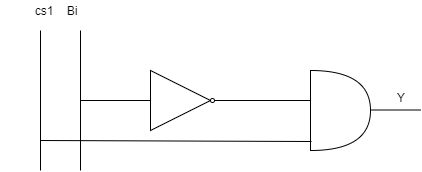
\includegraphics[width = 0.5\textwidth]{image/ckt1.png}
		\caption{
		$Y=CS_1\overline{B_i}$
		}
		\label{fig:ckt1}
		
	\end{figure}
	%--------------------------------------------------------arithmetic
	
	%--------------------------------------------------------logic
	\section{Design of Arithmetic Logic Unit}
	\textbf{Truth Table : Logical Operations}
		\begin{center}
		\begin{tabular}{ |c|c|c|c|c|c|c| } 
			\hline
			$cs_2$ & $cs_1$ & $cs_0$ & $x_i$ & $y_i$ & $f_i=X_i \oplus Y_i$ & Operation \\
			\hline
			
			\hline
			1 & 0 & 0 & $A_i$ & $0$ & $A_i$ & OR \\
			\hline
			
			\hline
			1 & 0 & 1 & $A_i$ & $0$ & $A_i+1$ & OR \\
			\hline
			
			\hline
			1 & 1 & 0 & $A_i$ & $B_i$ & $A_i-B_i-1$ & AND \\
			\hline
			
			\hline
			1 & 1 & 1 & $A_i$ & $B_i$ & $A_i-B_i$ & AND\\
			\hline
		\end{tabular}
	\end{center}

	\textbf{Explanation:}\newline
	we can't modify $Y_i$ because that would change the arithmetic operations
	and neither can omit $A_i$ in any input, So we change $X_i$,\newline
	Let,

	$X_i=A_i+K_i$ \newline
	$F_i=X_i \oplus Y_i$ \newline
	$F_i=X_i \oplus 0$ \newline
	$F_i=X_i$ \newline
	$F_i=A_i+K_i$\newline
	
	But the desired output is $A_i+B_i$. So putting $K_i=B_i$ \newline
	$F_i=X_i \oplus Y_i$\newline
	$F_i=(A_i \oplus K_i) \oplus \overline{B_i}$\newline
	$F_i=(A_i \oplus K_i)B_i + \overline{(A_i \oplus K_i)} .\overline{B_i}$\newline
	$F_i=A_iB_i + K_iB_i + \overline{A_i}.\overline{K_i}.\overline{B_i}$ \newline Here our desired operation is $A_iB_i$ \newline
	So, $A_iB_i + K_iB_i + \overline{A_i}.\overline{K_i}.\overline{B_i} = A_iB_i$\newline if $K_i=\overline{B_i}$	Then $F_i=A_iB_i$\newline
	So we need $K_i=B_i$ when we will do OR operation and $K_i=\overline{B_i}$ for AND operation.
	
	\begin{center}
		\begin{tabular}{|c|c|c|c|}
			\hline
			$cs_2$ & $cs_1$ & $cs_0$ & $B$ \\
			\hline
			
			\hline
			$1$ & $0$ & $0$ & $B_i$ \\
			\hline
			
			\hline
			$1$ & $0$ & $1$ & $B_i$ \\
			\hline
			
			\hline
			$1$ & $1$ & $0$ & $\overline{B_i}$ \\
			\hline
			
			\hline
			$1$ & $1$ & $1$ & $\overline{B_i}$ \\
			\hline
		\end{tabular}
	\end{center}
	So from the truth table we can derive, \newline
	$X_i=A_i+CS_2(\overline{CS_1}.B(CS_0 + \overline{CS_0})+CS_1.\overline{B_i}(CS_0 + \overline{CS_0})) )$ \newline
		$X_i=A_i+CS_2(CS_1\oplus B_i)$ \newline
	
	\begin{figure}[h]
		\centering
		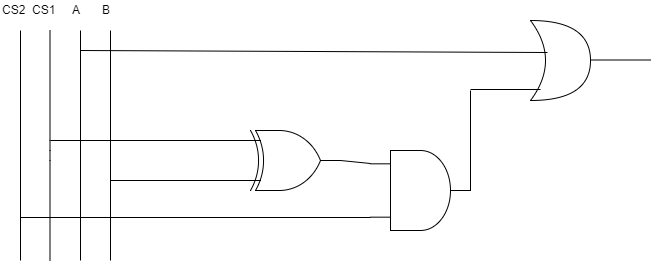
\includegraphics[width = 0.5\textwidth]{image/ckt2.png}
		\caption{
				$X_i=A_i+CS_2(CS_1\oplus B_i)$ \newline
		}
		\label{fig:ckt1}
		
	\end{figure}

	\section{Final Diagram}
		$X_i=A_i+CS_2(\overline{CS_1}.B(CS_0 + \overline{CS_0})+CS_1.\overline{B_i}(CS_0 + \overline{CS_0})) )$ \newline
		$X_i=A_i+CS_2(CS_1\oplus B_i)$ \newline
	$Y=CS_1\overline{B_i}$\newline
	$C_{out}=\overline{CS_2}.C_i$ 
	
	
	%--------------------------------------------------------logic	
\end{document}
